\documentclass{beamer}
%\documentclass[aspectratio=169]{beamer}
%
\mode<presentation>
{
  \usetheme{default}      
  \usecolortheme{default}
  \usefonttheme{default} 
  \setbeamertemplate{navigation symbols}{}
  \setbeamertemplate{caption}[numbered]
} 

\usepackage[english]{babel}
\usepackage[utf8x]{inputenc}

\title[Classification]{Introduction to Machine Learning}
\subtitle{Lecture 3: Regression}
\author{Alexis Zubiolo\newline\texttt{alexis.zubiolo@gmail.com}}
\institute{Data Science Team Lead @ Adcash}
\date{\today}

\begin{document}

\begin{frame}
  \titlepage
\end{frame}

\begin{frame}{Before we start}
Would you be interested in a more advanced course? I can propose 
\begin{itemize}
	\item Machine learning from scratch (how to implement an ML algorithm with no library)
	\item A more advanced version of this course (with more theoretical technical details)
	\item Large-scale machine learning
\end{itemize}
\end{frame}

\begin{frame}{Regression in Machine Learning}
This lecture is about regression in Machine learning.
\vfill
\textbf{Reminder}: In regression, the output $y$ is \textbf{continous}.
\vfill
\textbf{Example}:
\begin{itemize}
	\item \textbf{Price estimation}: $y =$ price (\textit{e.g.} 50000 BGN for a house)
	\item \textbf{Predicting the future} (\textit{e.g.} weather forecast): $y =$ temperature or amount of rain 
\end{itemize}
\end{frame}

\begin{frame}{Regression in Machine Learning: Applications}
Domains of application:
\begin{itemize}
	\item Price estimation/prediction
	\item Weather forecast
	\item Production quantity estimation
	\item Stock option price prediction
	\item Fit statistical model to data
	\item Physics \& chemistry
	\item \ldots{} and others
\end{itemize}
\end{frame}
%
\begin{frame}{Linear and polynomial regression}
Purpose of regression: \textbf{approximate solutions} of \textbf{overdetermined systems}.
\vfill
\begin{figure}
\centering
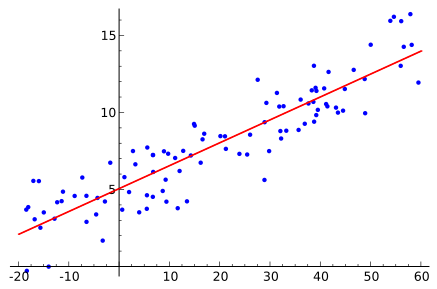
\includegraphics[width=0.70\textwidth]{images/2d_regression.png}
\end{figure}
\vfill
In this course, we will see
\begin{itemize}
	\item Linear regression
	\item Polynomial regression
\end{itemize}
\end{frame}
%
\begin{frame}
\begin{center}
\Huge{Linear regression}
\end{center}
\end{frame}
%
\begin{frame}{Linear regression}
Principal components:
\begin{itemize}
	\item Old problem (least-squares method usually credited to Carl Friedrich Gauss in 1795)
	\item Several ways to approximate the data
	\begin{itemize}
		\item Linear model
		\item Polynomial model (remember kernels from SVMs)
		\item Fit a distribution
		\item \ldots
	\end{itemize}
	\item Several ways to formulate the problem
	\begin{itemize}
		\item Least Squares
		\item Support Vector regression
		\item \ldots
	\end{itemize}
	\item Several ways to solve the problem
\end{itemize}
\end{frame}

\begin{frame}{Linear regression with ordinary least-squares}
\textbf{Linear} regression: Estimate $y$ as a \textbf{linear} function of $x$:
$$ \hat{y} = w^T x$$
\end{frame}

\begin{frame}

\begin{table}
\centering
\begin{tabular}{r|r|r}
living area (m$^2$) &  \textbf{\# bedrooms} & price (1000's euros) \\\hline
50 & \textbf{1} & 30\\
76 & \textbf{2} & 48\\
26 & \textbf{1} & 12\\
102 & \textbf{3} & 90\\
\pause
61 & \textbf{2} & ?
\end{tabular}
\end{table}

\end{frame}

\begin{frame}{Variable standardisation}
Variables have various magnitudes. Example:
\begin{itemize}
	\item Living area: Up to a few hundreds m$^2$
	\item Price: Up to a few 100 000s BGN (and even more)
\end{itemize}
\vfill
\pause
It is possible to calculate the \textbf{standard score} z of a variable x
$$ z = \dfrac{x - \mu}{\sigma}$$
where
\begin{itemize}
	\item $\mu$ is the mean of the variable
	\item $\sigma$ is its standard deviation
\end{itemize}
\pause
\vfill
Another option: Scale between 0 and 1
$$ z = \dfrac{x - \min}{\max - \min}$$
\end{frame}

\begin{frame}{Overfitting and underfitting }
$$ y = \cos \left( \dfrac{3\pi}{2} x \right) + \text{noise}$$
\begin{figure}
\centering
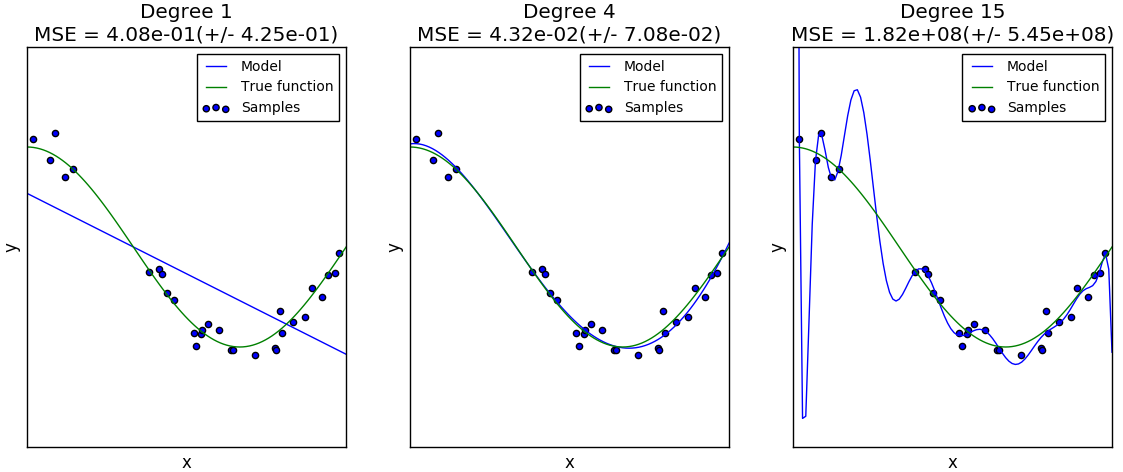
\includegraphics[width=\textwidth]{images/over_under_fitting.png}
\end{figure}
\end{frame}

\begin{frame}{Parameter selection}
Parameter selection plays a key role in the regression performance.
\end{frame}

\begin{frame}{Fitting a distribution}

\end{frame}

\begin{frame}
\begin{center}
\Huge{Thank you! Questions?}
\end{center}
\end{frame}

\end{document}